\documentclass[1p]{elsarticle_modified}
%\bibliographystyle{elsarticle-num}

%\usepackage[colorlinks]{hyperref}
%\usepackage{abbrmath_seonhwa} %\Abb, \Ascr, \Acal ,\Abf, \Afrak
\usepackage{amsfonts}
\usepackage{amssymb}
\usepackage{amsmath}
\usepackage{amsthm}
\usepackage{scalefnt}
\usepackage{amsbsy}
\usepackage{kotex}
\usepackage{caption}
\usepackage{subfig}
\usepackage{color}
\usepackage{graphicx}
\usepackage{xcolor} %% white, black, red, green, blue, cyan, magenta, yellow
\usepackage{float}
\usepackage{setspace}
\usepackage{hyperref}

\usepackage{tikz}
\usetikzlibrary{arrows}

\usepackage{multirow}
\usepackage{array} % fixed length table
\usepackage{hhline}

%%%%%%%%%%%%%%%%%%%%%
\makeatletter
\renewcommand*\env@matrix[1][\arraystretch]{%
	\edef\arraystretch{#1}%
	\hskip -\arraycolsep
	\let\@ifnextchar\new@ifnextchar
	\array{*\c@MaxMatrixCols c}}
\makeatother %https://tex.stackexchange.com/questions/14071/how-can-i-increase-the-line-spacing-in-a-matrix
%%%%%%%%%%%%%%%

\usepackage[normalem]{ulem}

\newcommand{\msout}[1]{\ifmmode\text{\sout{\ensuremath{#1}}}\else\sout{#1}\fi}
%SOURCE: \msout is \stkout macro in https://tex.stackexchange.com/questions/20609/strikeout-in-math-mode

\newcommand{\cancel}[1]{
	\ifmmode
	{\color{red}\msout{#1}}
	\else
	{\color{red}\sout{#1}}
	\fi
}

\newcommand{\add}[1]{
	{\color{blue}\uwave{#1}}
}

\newcommand{\replace}[2]{
	\ifmmode
	{\color{red}\msout{#1}}{\color{blue}\uwave{#2}}
	\else
	{\color{red}\sout{#1}}{\color{blue}\uwave{#2}}
	\fi
}

\newcommand{\Sol}{\mathcal{S}} %segment
\newcommand{\D}{D} %diagram
\newcommand{\A}{\mathcal{A}} %arc


%%%%%%%%%%%%%%%%%%%%%%%%%%%%%5 test

\def\sl{\operatorname{\textup{SL}}(2,\Cbb)}
\def\psl{\operatorname{\textup{PSL}}(2,\Cbb)}
\def\quan{\mkern 1mu \triangleright \mkern 1mu}

\theoremstyle{definition}
\newtheorem{thm}{Theorem}[section]
\newtheorem{prop}[thm]{Proposition}
\newtheorem{lem}[thm]{Lemma}
\newtheorem{ques}[thm]{Question}
\newtheorem{cor}[thm]{Corollary}
\newtheorem{defn}[thm]{Definition}
\newtheorem{exam}[thm]{Example}
\newtheorem{rmk}[thm]{Remark}
\newtheorem{alg}[thm]{Algorithm}

\newcommand{\I}{\sqrt{-1}}
\begin{document}

%\begin{frontmatter}
%
%\title{Boundary parabolic representations of knots up to 8 crossings}
%
%%% Group authors per affiliation:
%\author{Yunhi Cho} 
%\address{Department of Mathematics, University of Seoul, Seoul, Korea}
%\ead{yhcho@uos.ac.kr}
%
%
%\author{Seonhwa Kim} %\fnref{s_kim}}
%\address{Center for Geometry and Physics, Institute for Basic Science, Pohang, 37673, Korea}
%\ead{ryeona17@ibs.re.kr}
%
%\author{Hyuk Kim}
%\address{Department of Mathematical Sciences, Seoul National University, Seoul 08826, Korea}
%\ead{hyukkim@snu.ac.kr}
%
%\author{Seokbeom Yoon}
%\address{Department of Mathematical Sciences, Seoul National University, Seoul, 08826,  Korea}
%\ead{sbyoon15@snu.ac.kr}
%
%\begin{abstract}
%We find all boundary parabolic representation of knots up to 8 crossings.
%
%\end{abstract}
%\begin{keyword}
%    \MSC[2010] 57M25 
%\end{keyword}
%
%\end{frontmatter}

%\linenumbers
%\tableofcontents
%
\newcommand\colored[1]{\textcolor{white}{\rule[-0.35ex]{0.8em}{1.4ex}}\kern-0.8em\color{red} #1}%
%\newcommand\colored[1]{\textcolor{white}{ #1}\kern-2.17ex	\textcolor{white}{ #1}\kern-1.81ex	\textcolor{white}{ #1}\kern-2.15ex\color{red}#1	}

{\Large $\underline{12a_{1060}~(K12a_{1060})}$}

\setlength{\tabcolsep}{10pt}
\renewcommand{\arraystretch}{1.6}
\vspace{1cm}\begin{tabular}{m{100pt}>{\centering\arraybackslash}m{274pt}}
\multirow{5}{120pt}{
	\centering
	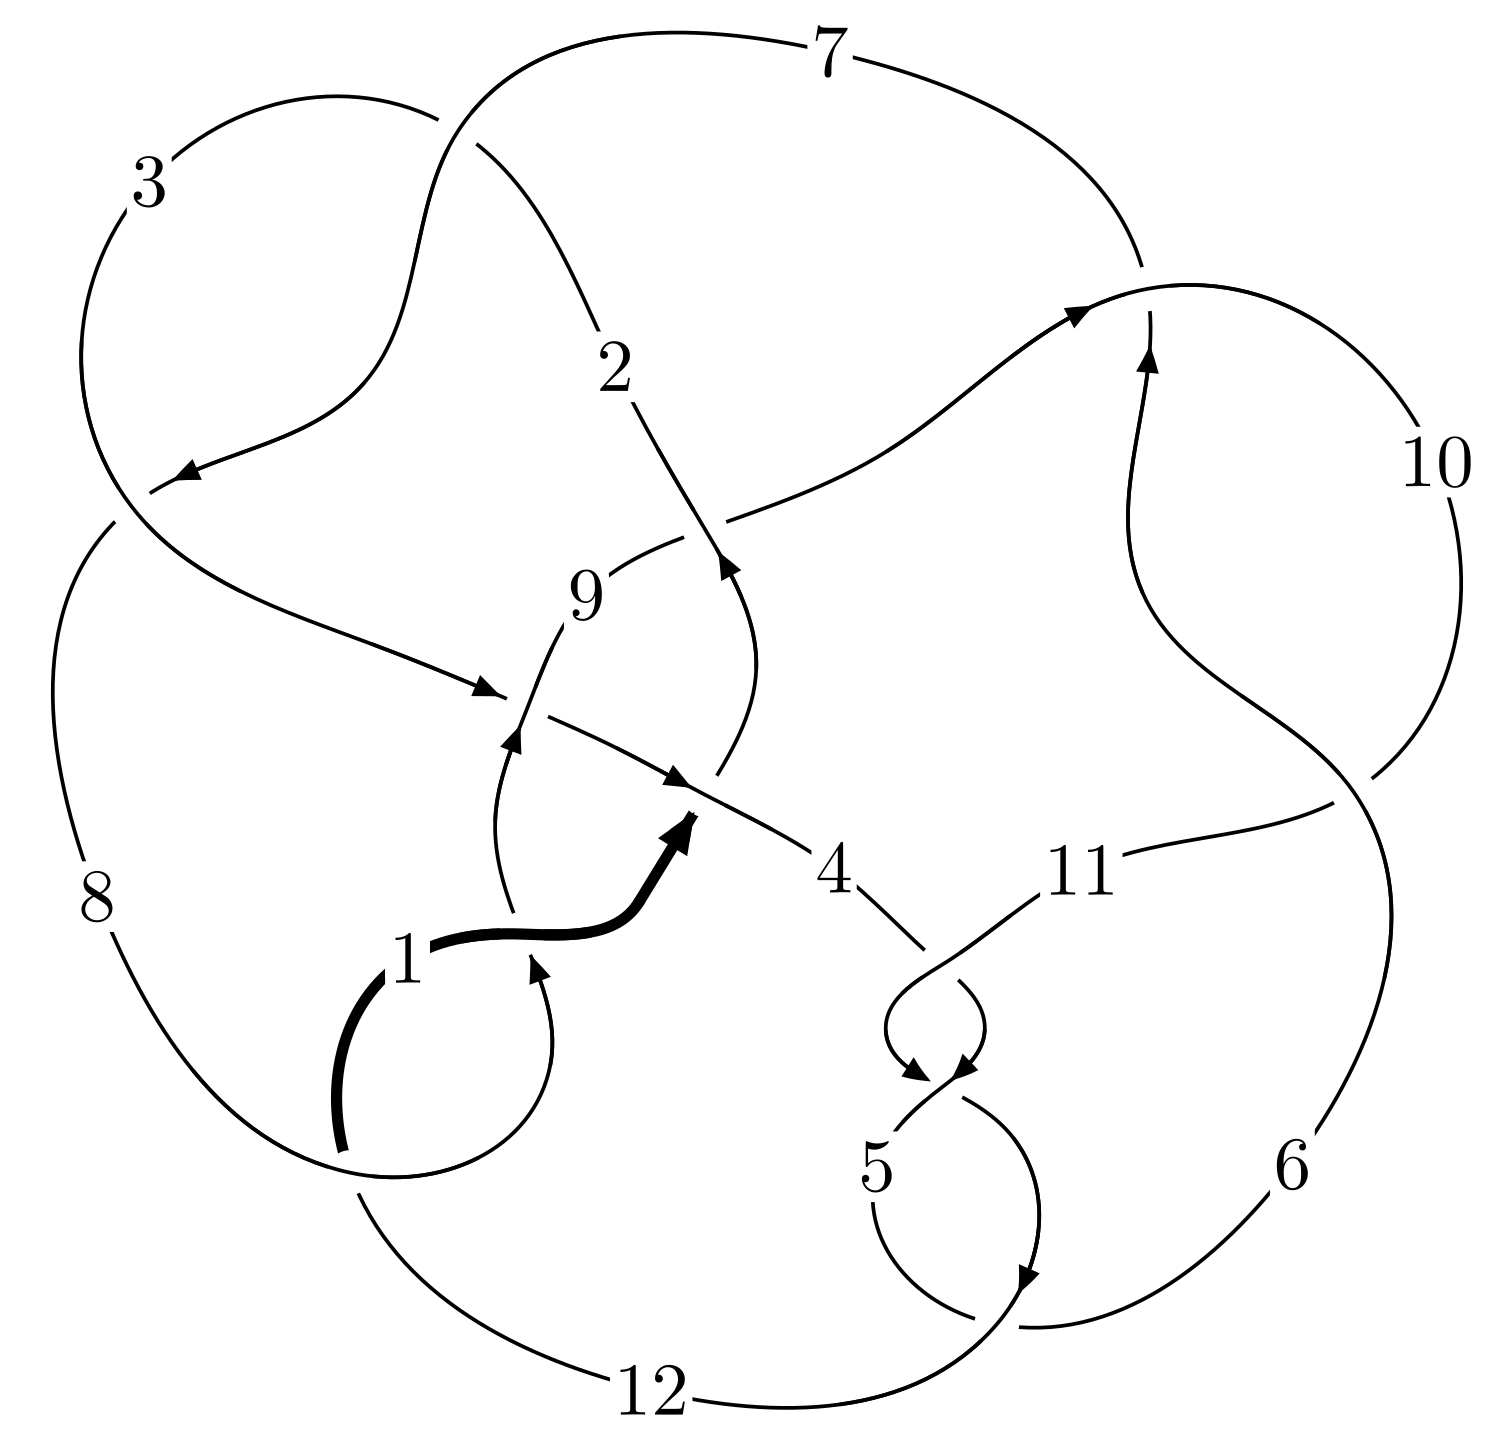
\includegraphics[width=112pt]{../../../GIT/diagram.site/Diagrams/png/1861_12a_1060.png}\\
\ \ \ A knot diagram\footnotemark}&
\allowdisplaybreaks
\textbf{Linearized knot diagam} \\
\cline{2-2}
 &
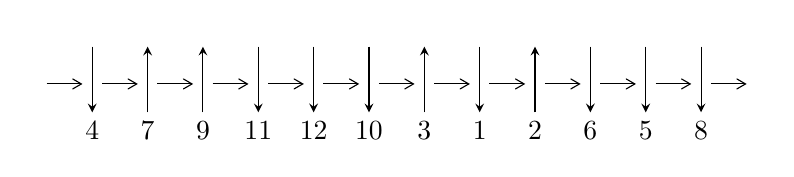
\begin{tikzpicture}[x=20pt, y=17pt]
	% nodes
	\node (C0) at (0, 0) {};
	\node (C1) at (1, 0) {};
	\node (C1U) at (1, +1) {};
	\node (C1D) at (1, -1) {4};

	\node (C2) at (2, 0) {};
	\node (C2U) at (2, +1) {};
	\node (C2D) at (2, -1) {7};

	\node (C3) at (3, 0) {};
	\node (C3U) at (3, +1) {};
	\node (C3D) at (3, -1) {9};

	\node (C4) at (4, 0) {};
	\node (C4U) at (4, +1) {};
	\node (C4D) at (4, -1) {11};

	\node (C5) at (5, 0) {};
	\node (C5U) at (5, +1) {};
	\node (C5D) at (5, -1) {12};

	\node (C6) at (6, 0) {};
	\node (C6U) at (6, +1) {};
	\node (C6D) at (6, -1) {10};

	\node (C7) at (7, 0) {};
	\node (C7U) at (7, +1) {};
	\node (C7D) at (7, -1) {3};

	\node (C8) at (8, 0) {};
	\node (C8U) at (8, +1) {};
	\node (C8D) at (8, -1) {1};

	\node (C9) at (9, 0) {};
	\node (C9U) at (9, +1) {};
	\node (C9D) at (9, -1) {2};

	\node (C10) at (10, 0) {};
	\node (C10U) at (10, +1) {};
	\node (C10D) at (10, -1) {6};

	\node (C11) at (11, 0) {};
	\node (C11U) at (11, +1) {};
	\node (C11D) at (11, -1) {5};

	\node (C12) at (12, 0) {};
	\node (C12U) at (12, +1) {};
	\node (C12D) at (12, -1) {8};
	\node (C13) at (13, 0) {};

	% arrows
	\draw[->,>={angle 60}]
	(C0) edge (C1) (C1) edge (C2) (C2) edge (C3) (C3) edge (C4) (C4) edge (C5) (C5) edge (C6) (C6) edge (C7) (C7) edge (C8) (C8) edge (C9) (C9) edge (C10) (C10) edge (C11) (C11) edge (C12) (C12) edge (C13) ;	\draw[->,>=stealth]
	(C1U) edge (C1D) (C2D) edge (C2U) (C3D) edge (C3U) (C4U) edge (C4D) (C5U) edge (C5D) (C6U) edge (C6D) (C7D) edge (C7U) (C8U) edge (C8D) (C9D) edge (C9U) (C10U) edge (C10D) (C11U) edge (C11D) (C12U) edge (C12D) ;
	\end{tikzpicture} \\
\hhline{~~} \\& 
\textbf{Solving Sequence} \\ \cline{2-2} 
 &
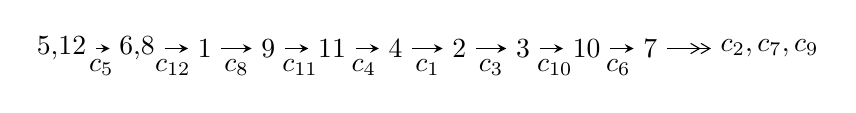
\begin{tikzpicture}[x=23pt, y=7pt]
	% node
	\node (A0) at (-1/8, 0) {5,12};
	\node (A1) at (17/16, 0) {6,8};
	\node (A2) at (17/8, 0) {1};
	\node (A3) at (25/8, 0) {9};
	\node (A4) at (33/8, 0) {11};
	\node (A5) at (41/8, 0) {4};
	\node (A6) at (49/8, 0) {2};
	\node (A7) at (57/8, 0) {3};
	\node (A8) at (65/8, 0) {10};
	\node (A9) at (73/8, 0) {7};
	\node (C1) at (1/2, -1) {$c_{5}$};
	\node (C2) at (13/8, -1) {$c_{12}$};
	\node (C3) at (21/8, -1) {$c_{8}$};
	\node (C4) at (29/8, -1) {$c_{11}$};
	\node (C5) at (37/8, -1) {$c_{4}$};
	\node (C6) at (45/8, -1) {$c_{1}$};
	\node (C7) at (53/8, -1) {$c_{3}$};
	\node (C8) at (61/8, -1) {$c_{10}$};
	\node (C9) at (69/8, -1) {$c_{6}$};
	\node (A10) at (11, 0) {$c_{2},c_{7},c_{9}$};

	% edge
	\draw[->,>=stealth]	
	(A0) edge (A1) (A1) edge (A2) (A2) edge (A3) (A3) edge (A4) (A4) edge (A5) (A5) edge (A6) (A6) edge (A7) (A7) edge (A8) (A8) edge (A9) ;
	\draw[->>,>={angle 60}]	
	(A9) edge (A10);
\end{tikzpicture} \\ 

\end{tabular} \\

\footnotetext{
The image of knot diagram is generated by the software ``\textbf{Draw programme}" developed by Andrew Bartholomew(\url{http://www.layer8.co.uk/maths/draw/index.htm\#Running-draw}), where we modified some parts for our purpose(\url{https://github.com/CATsTAILs/LinksPainter}).
}\phantom \\ \newline 
\centering \textbf{Ideals for irreducible components\footnotemark of $X_{\text{par}}$} 
 
\begin{align*}
I^u_{1}&=\langle 
-2.57346\times10^{89} u^{110}+1.88636\times10^{89} u^{109}+\cdots+1.74794\times10^{88} b+1.38329\times10^{89},\\
\phantom{I^u_{1}}&\phantom{= \langle  }-1.32168\times10^{89} u^{110}+1.72858\times10^{89} u^{109}+\cdots+1.74794\times10^{88} a+4.52966\times10^{89},\\
\phantom{I^u_{1}}&\phantom{= \langle  }u^{111}-2 u^{110}+\cdots-17 u+1\rangle \\
I^u_{2}&=\langle 
u^{20}- u^{19}+\cdots+b- u,\;- u^{20}+10 u^{18}+\cdots+a+1,\\
\phantom{I^u_{2}}&\phantom{= \langle  }u^{21}-10 u^{19}+42 u^{17}-92 u^{15}+99 u^{13}-14 u^{11}- u^{10}-78 u^9+5 u^8+60 u^7-9 u^6+9 u^5+6 u^4-18 u^3-1\rangle \\
I^u_{3}&=\langle 
b,\;a+1,\;u+1\rangle \\
\\
\end{align*}
\raggedright * 3 irreducible components of $\dim_{\mathbb{C}}=0$, with total 133 representations.\\
\footnotetext{All coefficients of polynomials are rational numbers. But the coefficients are sometimes approximated in decimal forms when there is not enough margin.}
\newpage
\renewcommand{\arraystretch}{1}
\centering \section*{I. $I^u_{1}= \langle -2.57\times10^{89} u^{110}+1.89\times10^{89} u^{109}+\cdots+1.75\times10^{88} b+1.38\times10^{89},\;-1.32\times10^{89} u^{110}+1.73\times10^{89} u^{109}+\cdots+1.75\times10^{88} a+4.53\times10^{89},\;u^{111}-2 u^{110}+\cdots-17 u+1 \rangle$}
\flushleft \textbf{(i) Arc colorings}\\
\begin{tabular}{m{7pt} m{180pt} m{7pt} m{180pt} }
\flushright $a_{5}=$&$\begin{pmatrix}1\\0\end{pmatrix}$ \\
\flushright $a_{12}=$&$\begin{pmatrix}0\\u\end{pmatrix}$ \\
\flushright $a_{6}=$&$\begin{pmatrix}1\\u^2\end{pmatrix}$ \\
\flushright $a_{8}=$&$\begin{pmatrix}7.56139 u^{110}-9.88923 u^{109}+\cdots+305.838 u-25.9143\\14.7228 u^{110}-10.7919 u^{109}+\cdots+165.490 u-7.91382\end{pmatrix}$ \\
\flushright $a_{1}=$&$\begin{pmatrix}-0.131615 u^{110}+1.70010 u^{109}+\cdots-107.174 u+6.20078\\-8.70767 u^{110}+7.11868 u^{109}+\cdots-150.414 u+11.0406\end{pmatrix}$ \\
\flushright $a_{9}=$&$\begin{pmatrix}3.79909 u^{110}-4.42765 u^{109}+\cdots+61.8715 u-3.31532\\10.8836 u^{110}-8.05693 u^{109}+\cdots+113.483 u-5.21542\end{pmatrix}$ \\
\flushright $a_{11}=$&$\begin{pmatrix}u\\u\end{pmatrix}$ \\
\flushright $a_{4}=$&$\begin{pmatrix}- u^2+1\\- u^2\end{pmatrix}$ \\
\flushright $a_{2}=$&$\begin{pmatrix}3.46413 u^{110}-1.77921 u^{109}+\cdots-21.8214 u-0.849966\\0.698222 u^{110}-0.237275 u^{109}+\cdots-24.5823 u+3.29697\end{pmatrix}$ \\
\flushright $a_{3}=$&$\begin{pmatrix}0.676351 u^{110}+1.22744 u^{109}+\cdots-101.879 u+5.95117\\-5.00556 u^{110}+4.25267 u^{109}+\cdots-104.692 u+8.32936\end{pmatrix}$ \\
\flushright $a_{10}=$&$\begin{pmatrix}- u^3+2 u\\- u^5+u^3+u\end{pmatrix}$ \\
\flushright $a_{7}=$&$\begin{pmatrix}u^6-3 u^4+2 u^2+1\\u^8-2 u^6+2 u^2\end{pmatrix}$\\&\end{tabular}
\flushleft \textbf{(ii) Obstruction class $= -1$}\\~\\
\flushleft \textbf{(iii) Cusp Shapes $= -13.5527 u^{110}+17.8532 u^{109}+\cdots-506.209 u+43.1001$}\\~\\
\newpage\renewcommand{\arraystretch}{1}
\flushleft \textbf{(iv) u-Polynomials at the component}\newline \\
\begin{tabular}{m{50pt}|m{274pt}}
Crossings & \hspace{64pt}u-Polynomials at each crossing \\
\hline $$\begin{aligned}c_{1}\end{aligned}$$&$\begin{aligned}
&u^{111}-16 u^{110}+\cdots+15 u+1
\end{aligned}$\\
\hline $$\begin{aligned}c_{2},c_{7}\end{aligned}$$&$\begin{aligned}
&u^{111}- u^{110}+\cdots+2080 u-1879
\end{aligned}$\\
\hline $$\begin{aligned}c_{3}\end{aligned}$$&$\begin{aligned}
&u^{111}- u^{110}+\cdots-49 u-5
\end{aligned}$\\
\hline $$\begin{aligned}c_{4},c_{5},c_{11}\end{aligned}$$&$\begin{aligned}
&u^{111}-2 u^{110}+\cdots-17 u+1
\end{aligned}$\\
\hline $$\begin{aligned}c_{6},c_{10}\end{aligned}$$&$\begin{aligned}
&u^{111}+3 u^{110}+\cdots-42277 u+3245
\end{aligned}$\\
\hline $$\begin{aligned}c_{8},c_{12}\end{aligned}$$&$\begin{aligned}
&u^{111}- u^{110}+\cdots-882 u+271
\end{aligned}$\\
\hline $$\begin{aligned}c_{9}\end{aligned}$$&$\begin{aligned}
&u^{111}+2 u^{110}+\cdots-123711 u+123383
\end{aligned}$\\
\hline
\end{tabular}\\~\\
\newpage\renewcommand{\arraystretch}{1}
\flushleft \textbf{(v) Riley Polynomials at the component}\newline \\
\begin{tabular}{m{50pt}|m{274pt}}
Crossings & \hspace{64pt}Riley Polynomials at each crossing \\
\hline $$\begin{aligned}c_{1}\end{aligned}$$&$\begin{aligned}
&y^{111}-4 y^{110}+\cdots+567 y-1
\end{aligned}$\\
\hline $$\begin{aligned}c_{2},c_{7}\end{aligned}$$&$\begin{aligned}
&y^{111}-85 y^{110}+\cdots+140050328 y-3530641
\end{aligned}$\\
\hline $$\begin{aligned}c_{3}\end{aligned}$$&$\begin{aligned}
&y^{111}- y^{110}+\cdots+881 y-25
\end{aligned}$\\
\hline $$\begin{aligned}c_{4},c_{5},c_{11}\end{aligned}$$&$\begin{aligned}
&y^{111}-92 y^{110}+\cdots+81 y-1
\end{aligned}$\\
\hline $$\begin{aligned}c_{6},c_{10}\end{aligned}$$&$\begin{aligned}
&y^{111}+87 y^{110}+\cdots+1070147809 y-10530025
\end{aligned}$\\
\hline $$\begin{aligned}c_{8},c_{12}\end{aligned}$$&$\begin{aligned}
&y^{111}-63 y^{110}+\cdots+624538 y-73441
\end{aligned}$\\
\hline $$\begin{aligned}c_{9}\end{aligned}$$&$\begin{aligned}
&y^{111}-34 y^{110}+\cdots+1350344005825 y-15223364689
\end{aligned}$\\
\hline
\end{tabular}\\~\\
\newpage\flushleft \textbf{(vi) Complex Volumes and Cusp Shapes}
$$\begin{array}{c|c|c}  
\text{Solutions to }I^u_{1}& \I (\text{vol} + \sqrt{-1}CS) & \text{Cusp shape}\\
 \hline 
\begin{aligned}
u &= -0.081166 + 0.904115 I \\
a &= -0.344352 + 0.904100 I \\
b &= -0.205252 + 0.162622 I\end{aligned}
 & \phantom{-}7.50937 + 0.87155 I & \phantom{-0.000000 } 0 \\ \hline\begin{aligned}
u &= -0.081166 - 0.904115 I \\
a &= -0.344352 - 0.904100 I \\
b &= -0.205252 - 0.162622 I\end{aligned}
 & \phantom{-}7.50937 - 0.87155 I & \phantom{-0.000000 } 0 \\ \hline\begin{aligned}
u &= -0.121934 + 0.870862 I \\
a &= -0.96469 - 1.31541 I \\
b &= -1.313980 + 0.103964 I\end{aligned}
 & \phantom{-}6.3847 + 13.3757 I & \phantom{-0.000000 } 0 \\ \hline\begin{aligned}
u &= -0.121934 - 0.870862 I \\
a &= -0.96469 + 1.31541 I \\
b &= -1.313980 - 0.103964 I\end{aligned}
 & \phantom{-}6.3847 - 13.3757 I & \phantom{-0.000000 } 0 \\ \hline\begin{aligned}
u &= \phantom{-}0.154867 + 0.858936 I \\
a &= -0.632403 + 0.871576 I \\
b &= -0.954252 - 0.565366 I\end{aligned}
 & \phantom{-}7.30644 - 4.30172 I & \phantom{-0.000000 } 0 \\ \hline\begin{aligned}
u &= \phantom{-}0.154867 - 0.858936 I \\
a &= -0.632403 - 0.871576 I \\
b &= -0.954252 + 0.565366 I\end{aligned}
 & \phantom{-}7.30644 + 4.30172 I & \phantom{-0.000000 } 0 \\ \hline\begin{aligned}
u &= -0.028698 + 0.855465 I \\
a &= -0.428888 - 0.916164 I \\
b &= -0.819599 - 0.897102 I\end{aligned}
 & \phantom{-}7.25427 + 3.69556 I & \phantom{-0.000000 } 0 \\ \hline\begin{aligned}
u &= -0.028698 - 0.855465 I \\
a &= -0.428888 + 0.916164 I \\
b &= -0.819599 + 0.897102 I\end{aligned}
 & \phantom{-}7.25427 - 3.69556 I & \phantom{-0.000000 } 0 \\ \hline\begin{aligned}
u &= \phantom{-}0.091469 + 0.844247 I \\
a &= -1.35317 - 0.57053 I \\
b &= -0.863472 - 0.322494 I\end{aligned}
 & \phantom{-}9.30952 - 6.81701 I & \phantom{-0.000000 } 0 \\ \hline\begin{aligned}
u &= \phantom{-}0.091469 - 0.844247 I \\
a &= -1.35317 + 0.57053 I \\
b &= -0.863472 + 0.322494 I\end{aligned}
 & \phantom{-}9.30952 + 6.81701 I & \phantom{-0.000000 } 0\\
 \hline 
 \end{array}$$\newpage$$\begin{array}{c|c|c}  
\text{Solutions to }I^u_{1}& \I (\text{vol} + \sqrt{-1}CS) & \text{Cusp shape}\\
 \hline 
\begin{aligned}
u &= \phantom{-}1.084410 + 0.417528 I \\
a &= \phantom{-}0.442236 - 0.588081 I \\
b &= \phantom{-}1.139120 + 0.401544 I\end{aligned}
 & \phantom{-}4.45379 - 0.29837 I & \phantom{-0.000000 } 0 \\ \hline\begin{aligned}
u &= \phantom{-}1.084410 - 0.417528 I \\
a &= \phantom{-}0.442236 + 0.588081 I \\
b &= \phantom{-}1.139120 - 0.401544 I\end{aligned}
 & \phantom{-}4.45379 + 0.29837 I & \phantom{-0.000000 } 0 \\ \hline\begin{aligned}
u &= \phantom{-}0.080213 + 0.812540 I \\
a &= \phantom{-}0.73148 - 1.41337 I \\
b &= \phantom{-}1.282600 + 0.337159 I\end{aligned}
 & \phantom{-}1.52000 - 6.82635 I & \phantom{-0.000000 -}0. + 6.98056 I \\ \hline\begin{aligned}
u &= \phantom{-}0.080213 - 0.812540 I \\
a &= \phantom{-}0.73148 + 1.41337 I \\
b &= \phantom{-}1.282600 - 0.337159 I\end{aligned}
 & \phantom{-}1.52000 + 6.82635 I & \phantom{-0.000000 } 0. - 6.98056 I \\ \hline\begin{aligned}
u &= -0.025621 + 0.814330 I \\
a &= \phantom{-}1.019490 - 0.056681 I \\
b &= \phantom{-}0.598997 - 0.234326 I\end{aligned}
 & \phantom{-}4.98734 + 2.15996 I & \phantom{-0.000000 } 0 \\ \hline\begin{aligned}
u &= -0.025621 - 0.814330 I \\
a &= \phantom{-}1.019490 + 0.056681 I \\
b &= \phantom{-}0.598997 + 0.234326 I\end{aligned}
 & \phantom{-}4.98734 - 2.15996 I & \phantom{-0.000000 } 0 \\ \hline\begin{aligned}
u &= -0.526631 + 0.615019 I \\
a &= -0.47851 - 1.41722 I \\
b &= -0.547739 - 0.056493 I\end{aligned}
 & \phantom{-}0.59594 - 4.27717 I & \phantom{-0.000000 } 0 \\ \hline\begin{aligned}
u &= -0.526631 - 0.615019 I \\
a &= -0.47851 + 1.41722 I \\
b &= -0.547739 + 0.056493 I\end{aligned}
 & \phantom{-}0.59594 + 4.27717 I & \phantom{-0.000000 } 0 \\ \hline\begin{aligned}
u &= -1.179560 + 0.191654 I \\
a &= -0.551352 - 0.599227 I \\
b &= -0.158132 - 0.269581 I\end{aligned}
 & -1.82003 + 0.41789 I & \phantom{-0.000000 } 0 \\ \hline\begin{aligned}
u &= -1.179560 - 0.191654 I \\
a &= -0.551352 + 0.599227 I \\
b &= -0.158132 + 0.269581 I\end{aligned}
 & -1.82003 - 0.41789 I & \phantom{-0.000000 } 0\\
 \hline 
 \end{array}$$\newpage$$\begin{array}{c|c|c}  
\text{Solutions to }I^u_{1}& \I (\text{vol} + \sqrt{-1}CS) & \text{Cusp shape}\\
 \hline 
\begin{aligned}
u &= \phantom{-}0.012361 + 0.800991 I \\
a &= -0.442197 - 1.094450 I \\
b &= -1.60146 + 0.33849 I\end{aligned}
 & \phantom{-}6.98387 - 0.56475 I & \phantom{-}1.87354 + 0. I\phantom{ +0.000000I} \\ \hline\begin{aligned}
u &= \phantom{-}0.012361 - 0.800991 I \\
a &= -0.442197 + 1.094450 I \\
b &= -1.60146 - 0.33849 I\end{aligned}
 & \phantom{-}6.98387 + 0.56475 I & \phantom{-}1.87354 + 0. I\phantom{ +0.000000I} \\ \hline\begin{aligned}
u &= \phantom{-}0.025664 + 0.796748 I \\
a &= -1.23003 + 1.38707 I \\
b &= -1.250320 + 0.348318 I\end{aligned}
 & \phantom{-}2.91600 - 3.82224 I & \phantom{-0.000000 -}0. + 4.16476 I \\ \hline\begin{aligned}
u &= \phantom{-}0.025664 - 0.796748 I \\
a &= -1.23003 - 1.38707 I \\
b &= -1.250320 - 0.348318 I\end{aligned}
 & \phantom{-}2.91600 + 3.82224 I & \phantom{-0.000000 } 0. - 4.16476 I \\ \hline\begin{aligned}
u &= -0.524571 + 0.585182 I \\
a &= \phantom{-}1.51013 + 0.68318 I \\
b &= \phantom{-}1.199700 - 0.103549 I\end{aligned}
 & \phantom{-}0.56437 + 8.53514 I & -4.00000 - 8.97660 I \\ \hline\begin{aligned}
u &= -0.524571 - 0.585182 I \\
a &= \phantom{-}1.51013 - 0.68318 I \\
b &= \phantom{-}1.199700 + 0.103549 I\end{aligned}
 & \phantom{-}0.56437 - 8.53514 I & -4.00000 + 8.97660 I \\ \hline\begin{aligned}
u &= \phantom{-}1.215450 + 0.034160 I \\
a &= -0.655743 - 0.538750 I \\
b &= -0.82287 - 1.17849 I\end{aligned}
 & -4.37066 - 2.85132 I & \phantom{-0.000000 } 0 \\ \hline\begin{aligned}
u &= \phantom{-}1.215450 - 0.034160 I \\
a &= -0.655743 + 0.538750 I \\
b &= -0.82287 + 1.17849 I\end{aligned}
 & -4.37066 + 2.85132 I & \phantom{-0.000000 } 0 \\ \hline\begin{aligned}
u &= -1.142310 + 0.441405 I \\
a &= \phantom{-}0.741922 + 0.868519 I \\
b &= \phantom{-}0.759050 - 0.116604 I\end{aligned}
 & \phantom{-}3.25745 - 8.68324 I & \phantom{-0.000000 } 0 \\ \hline\begin{aligned}
u &= -1.142310 - 0.441405 I \\
a &= \phantom{-}0.741922 - 0.868519 I \\
b &= \phantom{-}0.759050 + 0.116604 I\end{aligned}
 & \phantom{-}3.25745 + 8.68324 I & \phantom{-0.000000 } 0\\
 \hline 
 \end{array}$$\newpage$$\begin{array}{c|c|c}  
\text{Solutions to }I^u_{1}& \I (\text{vol} + \sqrt{-1}CS) & \text{Cusp shape}\\
 \hline 
\begin{aligned}
u &= \phantom{-}1.230730 + 0.129770 I \\
a &= \phantom{-}0.847427 + 0.283143 I \\
b &= \phantom{-}1.58411 - 1.41763 I\end{aligned}
 & -3.36757 - 4.77773 I & \phantom{-0.000000 } 0 \\ \hline\begin{aligned}
u &= \phantom{-}1.230730 - 0.129770 I \\
a &= \phantom{-}0.847427 - 0.283143 I \\
b &= \phantom{-}1.58411 + 1.41763 I\end{aligned}
 & -3.36757 + 4.77773 I & \phantom{-0.000000 } 0 \\ \hline\begin{aligned}
u &= \phantom{-}1.175080 + 0.397243 I \\
a &= -0.586512 - 0.763040 I \\
b &= -1.220310 + 0.097965 I\end{aligned}
 & \phantom{-}5.98708 + 2.35229 I & \phantom{-0.000000 } 0 \\ \hline\begin{aligned}
u &= \phantom{-}1.175080 - 0.397243 I \\
a &= -0.586512 + 0.763040 I \\
b &= -1.220310 - 0.097965 I\end{aligned}
 & \phantom{-}5.98708 - 2.35229 I & \phantom{-0.000000 } 0 \\ \hline\begin{aligned}
u &= \phantom{-}1.190270 + 0.350522 I \\
a &= -0.790578 + 0.647954 I \\
b &= -1.292380 - 0.473108 I\end{aligned}
 & -1.87331 + 2.61985 I & \phantom{-0.000000 } 0 \\ \hline\begin{aligned}
u &= \phantom{-}1.190270 - 0.350522 I \\
a &= -0.790578 - 0.647954 I \\
b &= -1.292380 + 0.473108 I\end{aligned}
 & -1.87331 - 2.61985 I & \phantom{-0.000000 } 0 \\ \hline\begin{aligned}
u &= \phantom{-}1.25185\phantom{ +0.000000I} \\
a &= \phantom{-}0.708215\phantom{ +0.000000I} \\
b &= \phantom{-}6.74388\phantom{ +0.000000I}\end{aligned}
 & -0.842109\phantom{ +0.000000I} & \phantom{-0.000000 } 0 \\ \hline\begin{aligned}
u &= -0.129040 + 0.730302 I \\
a &= \phantom{-}1.05885 + 1.38972 I \\
b &= \phantom{-}0.986008 + 0.154802 I\end{aligned}
 & \phantom{-}1.16972 + 3.02941 I & \phantom{-}0.581656 - 0.502191 I \\ \hline\begin{aligned}
u &= -0.129040 - 0.730302 I \\
a &= \phantom{-}1.05885 - 1.38972 I \\
b &= \phantom{-}0.986008 - 0.154802 I\end{aligned}
 & \phantom{-}1.16972 - 3.02941 I & \phantom{-}0.581656 + 0.502191 I \\ \hline\begin{aligned}
u &= -1.273620 + 0.076602 I \\
a &= -0.344736 - 0.467111 I \\
b &= \phantom{-}0.378767 + 0.209717 I\end{aligned}
 & -1.89161 + 0.63320 I & \phantom{-0.000000 } 0\\
 \hline 
 \end{array}$$\newpage$$\begin{array}{c|c|c}  
\text{Solutions to }I^u_{1}& \I (\text{vol} + \sqrt{-1}CS) & \text{Cusp shape}\\
 \hline 
\begin{aligned}
u &= -1.273620 - 0.076602 I \\
a &= -0.344736 + 0.467111 I \\
b &= \phantom{-}0.378767 - 0.209717 I\end{aligned}
 & -1.89161 - 0.63320 I & \phantom{-0.000000 } 0 \\ \hline\begin{aligned}
u &= -0.052261 + 0.719313 I \\
a &= \phantom{-}0.56144 + 1.85689 I \\
b &= \phantom{-}0.362230 + 0.199391 I\end{aligned}
 & \phantom{-}0.82057 + 2.54626 I & -3.60718 - 1.85382 I \\ \hline\begin{aligned}
u &= -0.052261 - 0.719313 I \\
a &= \phantom{-}0.56144 - 1.85689 I \\
b &= \phantom{-}0.362230 - 0.199391 I\end{aligned}
 & \phantom{-}0.82057 - 2.54626 I & -3.60718 + 1.85382 I \\ \hline\begin{aligned}
u &= -1.193200 + 0.465317 I \\
a &= -0.743332 + 0.064065 I \\
b &= -1.140780 - 0.292617 I\end{aligned}
 & \phantom{-}4.08896 + 4.00061 I & \phantom{-0.000000 } 0 \\ \hline\begin{aligned}
u &= -1.193200 - 0.465317 I \\
a &= -0.743332 - 0.064065 I \\
b &= -1.140780 + 0.292617 I\end{aligned}
 & \phantom{-}4.08896 - 4.00061 I & \phantom{-0.000000 } 0 \\ \hline\begin{aligned}
u &= \phantom{-}1.279440 + 0.124995 I \\
a &= -0.161902 - 0.194584 I \\
b &= -0.565355 - 1.026320 I\end{aligned}
 & -4.72872 - 2.56138 I & \phantom{-0.000000 } 0 \\ \hline\begin{aligned}
u &= \phantom{-}1.279440 - 0.124995 I \\
a &= -0.161902 + 0.194584 I \\
b &= -0.565355 + 1.026320 I\end{aligned}
 & -4.72872 + 2.56138 I & \phantom{-0.000000 } 0 \\ \hline\begin{aligned}
u &= -1.292750 + 0.034714 I \\
a &= \phantom{-}1.015070 - 0.528316 I \\
b &= \phantom{-}3.98562 - 0.36189 I\end{aligned}
 & -5.84342 + 3.49242 I & \phantom{-0.000000 } 0 \\ \hline\begin{aligned}
u &= -1.292750 - 0.034714 I \\
a &= \phantom{-}1.015070 + 0.528316 I \\
b &= \phantom{-}3.98562 + 0.36189 I\end{aligned}
 & -5.84342 - 3.49242 I & \phantom{-0.000000 } 0 \\ \hline\begin{aligned}
u &= -1.260740 + 0.296765 I \\
a &= -0.974598 - 0.581114 I \\
b &= -1.86237 - 1.41018 I\end{aligned}
 & -2.94268 + 1.10354 I & \phantom{-0.000000 } 0\\
 \hline 
 \end{array}$$\newpage$$\begin{array}{c|c|c}  
\text{Solutions to }I^u_{1}& \I (\text{vol} + \sqrt{-1}CS) & \text{Cusp shape}\\
 \hline 
\begin{aligned}
u &= -1.260740 - 0.296765 I \\
a &= -0.974598 + 0.581114 I \\
b &= -1.86237 + 1.41018 I\end{aligned}
 & -2.94268 - 1.10354 I & \phantom{-0.000000 } 0 \\ \hline\begin{aligned}
u &= \phantom{-}1.249570 + 0.345703 I \\
a &= \phantom{-}0.603798 - 0.930670 I \\
b &= -0.138375 - 0.619119 I\end{aligned}
 & -0.866061 - 0.293007 I & \phantom{-0.000000 } 0 \\ \hline\begin{aligned}
u &= \phantom{-}1.249570 - 0.345703 I \\
a &= \phantom{-}0.603798 + 0.930670 I \\
b &= -0.138375 + 0.619119 I\end{aligned}
 & -0.866061 + 0.293007 I & \phantom{-0.000000 } 0 \\ \hline\begin{aligned}
u &= -1.245970 + 0.359010 I \\
a &= \phantom{-}0.251361 - 0.577708 I \\
b &= \phantom{-}0.535194 - 0.101397 I\end{aligned}
 & \phantom{-}1.21676 + 2.06299 I & \phantom{-0.000000 } 0 \\ \hline\begin{aligned}
u &= -1.245970 - 0.359010 I \\
a &= \phantom{-}0.251361 + 0.577708 I \\
b &= \phantom{-}0.535194 + 0.101397 I\end{aligned}
 & \phantom{-}1.21676 - 2.06299 I & \phantom{-0.000000 } 0 \\ \hline\begin{aligned}
u &= \phantom{-}1.261040 + 0.349927 I \\
a &= -0.733629 - 0.044182 I \\
b &= -3.33029 + 2.29901 I\end{aligned}
 & \phantom{-}3.11498 - 3.57845 I & \phantom{-0.000000 } 0 \\ \hline\begin{aligned}
u &= \phantom{-}1.261040 - 0.349927 I \\
a &= -0.733629 + 0.044182 I \\
b &= -3.33029 - 2.29901 I\end{aligned}
 & \phantom{-}3.11498 + 3.57845 I & \phantom{-0.000000 } 0 \\ \hline\begin{aligned}
u &= -1.246320 + 0.399264 I \\
a &= \phantom{-}0.508156 + 0.407138 I \\
b &= -0.756437 + 0.263088 I\end{aligned}
 & \phantom{-}3.48869 + 0.80412 I & \phantom{-0.000000 } 0 \\ \hline\begin{aligned}
u &= -1.246320 - 0.399264 I \\
a &= \phantom{-}0.508156 - 0.407138 I \\
b &= -0.756437 - 0.263088 I\end{aligned}
 & \phantom{-}3.48869 - 0.80412 I & \phantom{-0.000000 } 0 \\ \hline\begin{aligned}
u &= -1.279340 + 0.353280 I \\
a &= \phantom{-}0.525220 + 0.477688 I \\
b &= \phantom{-}0.562776 - 1.283690 I\end{aligned}
 & \phantom{-}2.96533 + 4.72137 I & \phantom{-0.000000 } 0\\
 \hline 
 \end{array}$$\newpage$$\begin{array}{c|c|c}  
\text{Solutions to }I^u_{1}& \I (\text{vol} + \sqrt{-1}CS) & \text{Cusp shape}\\
 \hline 
\begin{aligned}
u &= -1.279340 - 0.353280 I \\
a &= \phantom{-}0.525220 - 0.477688 I \\
b &= \phantom{-}0.562776 + 1.283690 I\end{aligned}
 & \phantom{-}2.96533 - 4.72137 I & \phantom{-0.000000 } 0 \\ \hline\begin{aligned}
u &= -1.288410 + 0.349720 I \\
a &= -1.044060 + 0.445837 I \\
b &= -2.76410 - 1.24036 I\end{aligned}
 & -1.17957 + 7.95243 I & \phantom{-0.000000 } 0 \\ \hline\begin{aligned}
u &= -1.288410 - 0.349720 I \\
a &= -1.044060 - 0.445837 I \\
b &= -2.76410 + 1.24036 I\end{aligned}
 & -1.17957 - 7.95243 I & \phantom{-0.000000 } 0 \\ \hline\begin{aligned}
u &= \phantom{-}1.286620 + 0.362863 I \\
a &= \phantom{-}0.215037 + 0.603548 I \\
b &= \phantom{-}1.142380 + 0.534124 I\end{aligned}
 & \phantom{-}0.90063 - 6.39648 I & \phantom{-0.000000 } 0 \\ \hline\begin{aligned}
u &= \phantom{-}1.286620 - 0.362863 I \\
a &= \phantom{-}0.215037 - 0.603548 I \\
b &= \phantom{-}1.142380 - 0.534124 I\end{aligned}
 & \phantom{-}0.90063 + 6.39648 I & \phantom{-0.000000 } 0 \\ \hline\begin{aligned}
u &= \phantom{-}1.293240 + 0.390759 I \\
a &= -0.647394 - 0.092804 I \\
b &= -0.62304 + 1.60161 I\end{aligned}
 & \phantom{-}3.13563 - 8.16662 I & \phantom{-0.000000 } 0 \\ \hline\begin{aligned}
u &= \phantom{-}1.293240 - 0.390759 I \\
a &= -0.647394 + 0.092804 I \\
b &= -0.62304 - 1.60161 I\end{aligned}
 & \phantom{-}3.13563 + 8.16662 I & \phantom{-0.000000 } 0 \\ \hline\begin{aligned}
u &= \phantom{-}1.316370 + 0.314217 I \\
a &= \phantom{-}1.066920 - 0.099320 I \\
b &= \phantom{-}2.70014 - 1.07266 I\end{aligned}
 & -3.50013 - 6.30583 I & \phantom{-0.000000 } 0 \\ \hline\begin{aligned}
u &= \phantom{-}1.316370 - 0.314217 I \\
a &= \phantom{-}1.066920 + 0.099320 I \\
b &= \phantom{-}2.70014 + 1.07266 I\end{aligned}
 & -3.50013 + 6.30583 I & \phantom{-0.000000 } 0 \\ \hline\begin{aligned}
u &= -1.357420 + 0.123005 I \\
a &= \phantom{-}0.055884 - 0.790870 I \\
b &= \phantom{-}0.219826 - 1.339850 I\end{aligned}
 & -1.79691 + 5.42824 I & \phantom{-0.000000 } 0\\
 \hline 
 \end{array}$$\newpage$$\begin{array}{c|c|c}  
\text{Solutions to }I^u_{1}& \I (\text{vol} + \sqrt{-1}CS) & \text{Cusp shape}\\
 \hline 
\begin{aligned}
u &= -1.357420 - 0.123005 I \\
a &= \phantom{-}0.055884 + 0.790870 I \\
b &= \phantom{-}0.219826 + 1.339850 I\end{aligned}
 & -1.79691 - 5.42824 I & \phantom{-0.000000 } 0 \\ \hline\begin{aligned}
u &= -1.361100 + 0.084061 I \\
a &= -0.889472 + 0.178559 I \\
b &= -4.43462 - 0.05589 I\end{aligned}
 & -8.65164 + 5.28818 I & \phantom{-0.000000 } 0 \\ \hline\begin{aligned}
u &= -1.361100 - 0.084061 I \\
a &= -0.889472 - 0.178559 I \\
b &= -4.43462 + 0.05589 I\end{aligned}
 & -8.65164 - 5.28818 I & \phantom{-0.000000 } 0 \\ \hline\begin{aligned}
u &= -1.354580 + 0.206679 I \\
a &= \phantom{-}0.753347 + 0.206126 I \\
b &= \phantom{-}3.12215 + 1.39177 I\end{aligned}
 & -7.16797 + 1.58311 I & \phantom{-0.000000 } 0 \\ \hline\begin{aligned}
u &= -1.354580 - 0.206679 I \\
a &= \phantom{-}0.753347 - 0.206126 I \\
b &= \phantom{-}3.12215 - 1.39177 I\end{aligned}
 & -7.16797 - 1.58311 I & \phantom{-0.000000 } 0 \\ \hline\begin{aligned}
u &= -1.322880 + 0.358837 I \\
a &= \phantom{-}0.959315 - 0.094899 I \\
b &= \phantom{-}3.52906 + 1.42336 I\end{aligned}
 & -2.87719 + 11.04810 I & \phantom{-0.000000 } 0 \\ \hline\begin{aligned}
u &= -1.322880 - 0.358837 I \\
a &= \phantom{-}0.959315 + 0.094899 I \\
b &= \phantom{-}3.52906 - 1.42336 I\end{aligned}
 & -2.87719 - 11.04810 I & \phantom{-0.000000 } 0 \\ \hline\begin{aligned}
u &= \phantom{-}0.527747 + 0.332177 I \\
a &= \phantom{-}0.694115 + 0.501497 I \\
b &= \phantom{-}1.059300 + 0.321123 I\end{aligned}
 & \phantom{-}3.19985 + 0.32140 I & \phantom{-}1.59922 + 2.05291 I \\ \hline\begin{aligned}
u &= \phantom{-}0.527747 - 0.332177 I \\
a &= \phantom{-}0.694115 - 0.501497 I \\
b &= \phantom{-}1.059300 - 0.321123 I\end{aligned}
 & \phantom{-}3.19985 - 0.32140 I & \phantom{-}1.59922 - 2.05291 I \\ \hline\begin{aligned}
u &= \phantom{-}1.341820 + 0.311397 I \\
a &= \phantom{-}1.028620 + 0.219802 I \\
b &= \phantom{-}2.94137 - 1.00859 I\end{aligned}
 & -3.46066 - 6.81605 I & \phantom{-0.000000 } 0\\
 \hline 
 \end{array}$$\newpage$$\begin{array}{c|c|c}  
\text{Solutions to }I^u_{1}& \I (\text{vol} + \sqrt{-1}CS) & \text{Cusp shape}\\
 \hline 
\begin{aligned}
u &= \phantom{-}1.341820 - 0.311397 I \\
a &= \phantom{-}1.028620 - 0.219802 I \\
b &= \phantom{-}2.94137 + 1.00859 I\end{aligned}
 & -3.46066 + 6.81605 I & \phantom{-0.000000 } 0 \\ \hline\begin{aligned}
u &= \phantom{-}1.380850 + 0.001402 I \\
a &= -1.002190 + 0.099681 I \\
b &= -3.63865 + 0.11066 I\end{aligned}
 & -7.48663 + 0.05717 I & \phantom{-0.000000 } 0 \\ \hline\begin{aligned}
u &= \phantom{-}1.380850 - 0.001402 I \\
a &= -1.002190 - 0.099681 I \\
b &= -3.63865 - 0.11066 I\end{aligned}
 & -7.48663 - 0.05717 I & \phantom{-0.000000 } 0 \\ \hline\begin{aligned}
u &= -0.618101 + 0.029425 I \\
a &= -1.74047 + 0.02330 I \\
b &= -0.535160 - 0.050220 I\end{aligned}
 & -1.53250 + 0.00940 I & -7.61099 + 0.23089 I \\ \hline\begin{aligned}
u &= -0.618101 - 0.029425 I \\
a &= -1.74047 - 0.02330 I \\
b &= -0.535160 + 0.050220 I\end{aligned}
 & -1.53250 - 0.00940 I & -7.61099 - 0.23089 I \\ \hline\begin{aligned}
u &= -1.332360 + 0.374895 I \\
a &= -0.013321 + 0.926101 I \\
b &= -0.998412 + 0.993180 I\end{aligned}
 & \phantom{-}4.84444 + 11.19960 I & \phantom{-0.000000 } 0 \\ \hline\begin{aligned}
u &= -1.332360 - 0.374895 I \\
a &= -0.013321 - 0.926101 I \\
b &= -0.998412 - 0.993180 I\end{aligned}
 & \phantom{-}4.84444 - 11.19960 I & \phantom{-0.000000 } 0 \\ \hline\begin{aligned}
u &= \phantom{-}0.387681 + 0.471766 I \\
a &= \phantom{-}0.94998 + 1.12985 I \\
b &= \phantom{-}0.192196 - 0.091930 I\end{aligned}
 & \phantom{-}3.65065 - 3.48280 I & \phantom{-}1.08914 + 6.57604 I \\ \hline\begin{aligned}
u &= \phantom{-}0.387681 - 0.471766 I \\
a &= \phantom{-}0.94998 - 1.12985 I \\
b &= \phantom{-}0.192196 + 0.091930 I\end{aligned}
 & \phantom{-}3.65065 + 3.48280 I & \phantom{-}1.08914 - 6.57604 I \\ \hline\begin{aligned}
u &= \phantom{-}1.331550 + 0.416484 I \\
a &= \phantom{-}0.431825 - 0.390425 I \\
b &= \phantom{-}0.625797 - 0.534575 I\end{aligned}
 & \phantom{-}3.09221 - 5.59637 I & \phantom{-0.000000 } 0\\
 \hline 
 \end{array}$$\newpage$$\begin{array}{c|c|c}  
\text{Solutions to }I^u_{1}& \I (\text{vol} + \sqrt{-1}CS) & \text{Cusp shape}\\
 \hline 
\begin{aligned}
u &= \phantom{-}1.331550 - 0.416484 I \\
a &= \phantom{-}0.431825 + 0.390425 I \\
b &= \phantom{-}0.625797 + 0.534575 I\end{aligned}
 & \phantom{-}3.09221 + 5.59637 I & \phantom{-0.000000 } 0 \\ \hline\begin{aligned}
u &= \phantom{-}0.239442 + 0.553403 I \\
a &= \phantom{-}0.29215 - 1.63161 I \\
b &= \phantom{-}0.814891 + 0.000066 I\end{aligned}
 & -2.15238 + 1.18175 I & -5.85912 + 1.80919 I \\ \hline\begin{aligned}
u &= \phantom{-}0.239442 - 0.553403 I \\
a &= \phantom{-}0.29215 + 1.63161 I \\
b &= \phantom{-}0.814891 - 0.000066 I\end{aligned}
 & -2.15238 - 1.18175 I & -5.85912 - 1.80919 I \\ \hline\begin{aligned}
u &= \phantom{-}1.354290 + 0.385786 I \\
a &= -1.013040 - 0.215829 I \\
b &= -3.22338 + 1.21261 I\end{aligned}
 & \phantom{-}1.7439 - 17.8882 I & \phantom{-0.000000 } 0 \\ \hline\begin{aligned}
u &= \phantom{-}1.354290 - 0.385786 I \\
a &= -1.013040 + 0.215829 I \\
b &= -3.22338 - 1.21261 I\end{aligned}
 & \phantom{-}1.7439 + 17.8882 I & \phantom{-0.000000 } 0 \\ \hline\begin{aligned}
u &= -1.37149 + 0.37859 I \\
a &= -0.688647 + 0.081503 I \\
b &= -2.89193 - 0.66737 I\end{aligned}
 & \phantom{-}2.49624 + 8.75887 I & \phantom{-0.000000 } 0 \\ \hline\begin{aligned}
u &= -1.37149 - 0.37859 I \\
a &= -0.688647 - 0.081503 I \\
b &= -2.89193 + 0.66737 I\end{aligned}
 & \phantom{-}2.49624 - 8.75887 I & \phantom{-0.000000 } 0 \\ \hline\begin{aligned}
u &= \phantom{-}1.42545 + 0.14891 I \\
a &= \phantom{-}0.929723 + 0.271581 I \\
b &= \phantom{-}3.68084 - 0.20743 I\end{aligned}
 & -5.71189 - 10.93540 I & \phantom{-0.000000 } 0 \\ \hline\begin{aligned}
u &= \phantom{-}1.42545 - 0.14891 I \\
a &= \phantom{-}0.929723 - 0.271581 I \\
b &= \phantom{-}3.68084 + 0.20743 I\end{aligned}
 & -5.71189 + 10.93540 I & \phantom{-0.000000 } 0 \\ \hline\begin{aligned}
u &= \phantom{-}0.449955 + 0.306106 I \\
a &= -2.03754 + 0.58119 I \\
b &= -1.245410 - 0.306755 I\end{aligned}
 & -3.08409 - 4.01496 I & -8.48201 + 7.35166 I\\
 \hline 
 \end{array}$$\newpage$$\begin{array}{c|c|c}  
\text{Solutions to }I^u_{1}& \I (\text{vol} + \sqrt{-1}CS) & \text{Cusp shape}\\
 \hline 
\begin{aligned}
u &= \phantom{-}0.449955 - 0.306106 I \\
a &= -2.03754 - 0.58119 I \\
b &= -1.245410 + 0.306755 I\end{aligned}
 & -3.08409 + 4.01496 I & -8.48201 - 7.35166 I \\ \hline\begin{aligned}
u &= -0.105666 + 0.512091 I \\
a &= \phantom{-}0.97329 + 1.87270 I \\
b &= \phantom{-}0.490136 + 0.627445 I\end{aligned}
 & \phantom{-}0.52426 + 2.56205 I & \phantom{-}0.27637 - 5.10765 I \\ \hline\begin{aligned}
u &= -0.105666 - 0.512091 I \\
a &= \phantom{-}0.97329 - 1.87270 I \\
b &= \phantom{-}0.490136 - 0.627445 I\end{aligned}
 & \phantom{-}0.52426 - 2.56205 I & \phantom{-}0.27637 + 5.10765 I \\ \hline\begin{aligned}
u &= \phantom{-}1.47079 + 0.14608 I \\
a &= -0.745847 + 0.294962 I \\
b &= -2.71132 + 0.77604 I\end{aligned}
 & -5.95978 + 1.70857 I & \phantom{-0.000000 } 0 \\ \hline\begin{aligned}
u &= \phantom{-}1.47079 - 0.14608 I \\
a &= -0.745847 - 0.294962 I \\
b &= -2.71132 - 0.77604 I\end{aligned}
 & -5.95978 - 1.70857 I & \phantom{-0.000000 } 0 \\ \hline\begin{aligned}
u &= -1.50434\phantom{ +0.000000I} \\
a &= \phantom{-}0.492040\phantom{ +0.000000I} \\
b &= \phantom{-}2.97475\phantom{ +0.000000I}\end{aligned}
 & -3.63276\phantom{ +0.000000I} & \phantom{-0.000000 } 0 \\ \hline\begin{aligned}
u &= -0.225847 + 0.327044 I \\
a &= -0.800511 + 0.558951 I \\
b &= -0.020085 + 0.267612 I\end{aligned}
 & -0.235196 + 0.938220 I & -4.68352 - 7.13050 I \\ \hline\begin{aligned}
u &= -0.225847 - 0.327044 I \\
a &= -0.800511 - 0.558951 I \\
b &= -0.020085 - 0.267612 I\end{aligned}
 & -0.235196 - 0.938220 I & -4.68352 + 7.13050 I \\ \hline\begin{aligned}
u &= \phantom{-}0.151934 + 0.115584 I \\
a &= \phantom{-}6.77942 - 0.80780 I \\
b &= \phantom{-}0.686578 - 0.179927 I\end{aligned}
 & -1.43186 - 2.95721 I & -9.1241 + 11.4688 I \\ \hline\begin{aligned}
u &= \phantom{-}0.151934 - 0.115584 I \\
a &= \phantom{-}6.77942 + 0.80780 I \\
b &= \phantom{-}0.686578 + 0.179927 I\end{aligned}
 & -1.43186 + 2.95721 I & -9.1241 - 11.4688 I\\
 \hline 
 \end{array}$$\newpage$$\begin{array}{c|c|c}  
\text{Solutions to }I^u_{1}& \I (\text{vol} + \sqrt{-1}CS) & \text{Cusp shape}\\
 \hline 
\begin{aligned}
u &= \phantom{-}0.119052\phantom{ +0.000000I} \\
a &= -5.01443\phantom{ +0.000000I} \\
b &= \phantom{-}1.98261\phantom{ +0.000000I}\end{aligned}
 & \phantom{-}2.72207\phantom{ +0.000000I} & \phantom{-}12.4830\phantom{ +0.000000I}\\
 \hline 
 \end{array}$$\newpage\newpage\renewcommand{\arraystretch}{1}
\centering \section*{II. $I^u_{2}= \langle u^{20}- u^{19}+\cdots+b- u,\;- u^{20}+10 u^{18}+\cdots+a+1,\;u^{21}-10 u^{19}+\cdots-18 u^3-1 \rangle$}
\flushleft \textbf{(i) Arc colorings}\\
\begin{tabular}{m{7pt} m{180pt} m{7pt} m{180pt} }
\flushright $a_{5}=$&$\begin{pmatrix}1\\0\end{pmatrix}$ \\
\flushright $a_{12}=$&$\begin{pmatrix}0\\u\end{pmatrix}$ \\
\flushright $a_{6}=$&$\begin{pmatrix}1\\u^2\end{pmatrix}$ \\
\flushright $a_{8}=$&$\begin{pmatrix}u^{20}-10 u^{18}+\cdots-3 u-1\\- u^{20}+u^{19}+\cdots-6 u^2+u\end{pmatrix}$ \\
\flushright $a_{1}=$&$\begin{pmatrix}u^{19}+u^{18}+\cdots+5 u+2\\- u^{20}+3 u^{19}+\cdots- u+2\end{pmatrix}$ \\
\flushright $a_{9}=$&$\begin{pmatrix}- u^{19}+9 u^{17}+\cdots+3 u+1\\-2 u^{20}- u^{19}+\cdots+u-1\end{pmatrix}$ \\
\flushright $a_{11}=$&$\begin{pmatrix}u\\u\end{pmatrix}$ \\
\flushright $a_{4}=$&$\begin{pmatrix}- u^2+1\\- u^2\end{pmatrix}$ \\
\flushright $a_{2}=$&$\begin{pmatrix}u^{20}+u^{19}+\cdots+6 u+2\\u^{20}+3 u^{19}+\cdots+6 u^2+2\end{pmatrix}$ \\
\flushright $a_{3}=$&$\begin{pmatrix}u^{19}+u^{18}+\cdots+5 u+3\\3 u^{19}+u^{18}+\cdots- u+2\end{pmatrix}$ \\
\flushright $a_{10}=$&$\begin{pmatrix}- u^3+2 u\\- u^5+u^3+u\end{pmatrix}$ \\
\flushright $a_{7}=$&$\begin{pmatrix}u^6-3 u^4+2 u^2+1\\u^8-2 u^6+2 u^2\end{pmatrix}$\\&\end{tabular}
\flushleft \textbf{(ii) Obstruction class $= 1$}\\~\\
\flushleft \textbf{(iii) Cusp Shapes $= -12 u^{19}-2 u^{18}+100 u^{17}+17 u^{16}-336 u^{15}-58 u^{14}+535 u^{13}+92 u^{12}-271 u^{11}-41 u^{10}-324 u^9-56 u^8+442 u^7+40 u^6-28 u^5+46 u^4-134 u^3-32 u^2+12 u-14$}\\~\\
\newpage\renewcommand{\arraystretch}{1}
\flushleft \textbf{(iv) u-Polynomials at the component}\newline \\
\begin{tabular}{m{50pt}|m{274pt}}
Crossings & \hspace{64pt}u-Polynomials at each crossing \\
\hline $$\begin{aligned}c_{1}\end{aligned}$$&$\begin{aligned}
&u^{21}-2 u^{19}+\cdots-6 u+1
\end{aligned}$\\
\hline $$\begin{aligned}c_{2}\end{aligned}$$&$\begin{aligned}
&u^{21}+u^{20}+\cdots+u+1
\end{aligned}$\\
\hline $$\begin{aligned}c_{3}\end{aligned}$$&$\begin{aligned}
&u^{21}-2 u^{19}+\cdots+3 u^2+1
\end{aligned}$\\
\hline $$\begin{aligned}c_{4},c_{5}\end{aligned}$$&$\begin{aligned}
&u^{21}-10 u^{19}+\cdots-18 u^3-1
\end{aligned}$\\
\hline $$\begin{aligned}c_{6}\end{aligned}$$&$\begin{aligned}
&u^{21}+6 u^{19}+\cdots+3 u^2-1
\end{aligned}$\\
\hline $$\begin{aligned}c_{7}\end{aligned}$$&$\begin{aligned}
&u^{21}- u^{20}+\cdots+u-1
\end{aligned}$\\
\hline $$\begin{aligned}c_{8}\end{aligned}$$&$\begin{aligned}
&u^{21}- u^{20}+\cdots+u-1
\end{aligned}$\\
\hline $$\begin{aligned}c_{9}\end{aligned}$$&$\begin{aligned}
&u^{21}+3 u^{19}+\cdots-2 u^2+1
\end{aligned}$\\
\hline $$\begin{aligned}c_{10}\end{aligned}$$&$\begin{aligned}
&u^{21}+6 u^{19}+\cdots-3 u^2+1
\end{aligned}$\\
\hline $$\begin{aligned}c_{11}\end{aligned}$$&$\begin{aligned}
&u^{21}-10 u^{19}+\cdots-18 u^3+1
\end{aligned}$\\
\hline $$\begin{aligned}c_{12}\end{aligned}$$&$\begin{aligned}
&u^{21}+u^{20}+\cdots+u+1
\end{aligned}$\\
\hline
\end{tabular}\\~\\
\newpage\renewcommand{\arraystretch}{1}
\flushleft \textbf{(v) Riley Polynomials at the component}\newline \\
\begin{tabular}{m{50pt}|m{274pt}}
Crossings & \hspace{64pt}Riley Polynomials at each crossing \\
\hline $$\begin{aligned}c_{1}\end{aligned}$$&$\begin{aligned}
&y^{21}-4 y^{20}+\cdots+10 y-1
\end{aligned}$\\
\hline $$\begin{aligned}c_{2},c_{7}\end{aligned}$$&$\begin{aligned}
&y^{21}-21 y^{20}+\cdots+15 y-1
\end{aligned}$\\
\hline $$\begin{aligned}c_{3}\end{aligned}$$&$\begin{aligned}
&y^{21}-4 y^{20}+\cdots-6 y-1
\end{aligned}$\\
\hline $$\begin{aligned}c_{4},c_{5},c_{11}\end{aligned}$$&$\begin{aligned}
&y^{21}-20 y^{20}+\cdots+12 y^2-1
\end{aligned}$\\
\hline $$\begin{aligned}c_{6},c_{10}\end{aligned}$$&$\begin{aligned}
&y^{21}+12 y^{20}+\cdots+6 y-1
\end{aligned}$\\
\hline $$\begin{aligned}c_{8},c_{12}\end{aligned}$$&$\begin{aligned}
&y^{21}-15 y^{20}+\cdots+21 y-1
\end{aligned}$\\
\hline $$\begin{aligned}c_{9}\end{aligned}$$&$\begin{aligned}
&y^{21}+6 y^{20}+\cdots+4 y-1
\end{aligned}$\\
\hline
\end{tabular}\\~\\
\newpage\flushleft \textbf{(vi) Complex Volumes and Cusp Shapes}
$$\begin{array}{c|c|c}  
\text{Solutions to }I^u_{2}& \I (\text{vol} + \sqrt{-1}CS) & \text{Cusp shape}\\
 \hline 
\begin{aligned}
u &= -0.062614 + 0.857160 I \\
a &= \phantom{-}0.275352 + 0.744219 I \\
b &= \phantom{-}0.991659 + 0.241341 I\end{aligned}
 & \phantom{-}7.09483 + 2.69700 I & \phantom{-}0.204052 - 0.960418 I \\ \hline\begin{aligned}
u &= -0.062614 - 0.857160 I \\
a &= \phantom{-}0.275352 - 0.744219 I \\
b &= \phantom{-}0.991659 - 0.241341 I\end{aligned}
 & \phantom{-}7.09483 - 2.69700 I & \phantom{-}0.204052 + 0.960418 I \\ \hline\begin{aligned}
u &= -1.18462\phantom{ +0.000000I} \\
a &= \phantom{-}0.514078\phantom{ +0.000000I} \\
b &= -3.17275\phantom{ +0.000000I}\end{aligned}
 & -0.0653881\phantom{ +0.000000I} & \phantom{-}2.89470\phantom{ +0.000000I} \\ \hline\begin{aligned}
u &= \phantom{-}1.235030 + 0.104057 I \\
a &= -0.770955 - 0.434248 I \\
b &= -1.68506 - 0.31727 I\end{aligned}
 & -4.45553 - 3.99750 I & -8.33700 + 7.35069 I \\ \hline\begin{aligned}
u &= \phantom{-}1.235030 - 0.104057 I \\
a &= -0.770955 + 0.434248 I \\
b &= -1.68506 + 0.31727 I\end{aligned}
 & -4.45553 + 3.99750 I & -8.33700 - 7.35069 I \\ \hline\begin{aligned}
u &= \phantom{-}1.234780 + 0.272929 I \\
a &= \phantom{-}0.736844 - 0.846584 I \\
b &= \phantom{-}0.398323 - 0.870978 I\end{aligned}
 & -2.77607 + 0.23467 I & -9.48318 - 3.28637 I \\ \hline\begin{aligned}
u &= \phantom{-}1.234780 - 0.272929 I \\
a &= \phantom{-}0.736844 + 0.846584 I \\
b &= \phantom{-}0.398323 + 0.870978 I\end{aligned}
 & -2.77607 - 0.23467 I & -9.48318 + 3.28637 I \\ \hline\begin{aligned}
u &= -1.212920 + 0.392860 I \\
a &= -0.439696 - 0.262167 I \\
b &= \phantom{-}0.203010 + 0.888489 I\end{aligned}
 & \phantom{-}3.55654 + 1.79152 I & -2.35096 - 2.63279 I \\ \hline\begin{aligned}
u &= -1.212920 - 0.392860 I \\
a &= -0.439696 + 0.262167 I \\
b &= \phantom{-}0.203010 - 0.888489 I\end{aligned}
 & \phantom{-}3.55654 - 1.79152 I & -2.35096 + 2.63279 I \\ \hline\begin{aligned}
u &= \phantom{-}0.072517 + 0.710236 I \\
a &= -1.26753 + 1.64767 I \\
b &= -1.045360 + 0.236003 I\end{aligned}
 & \phantom{-}0.77767 - 3.77401 I & -4.35410 + 8.39040 I\\
 \hline 
 \end{array}$$\newpage$$\begin{array}{c|c|c}  
\text{Solutions to }I^u_{2}& \I (\text{vol} + \sqrt{-1}CS) & \text{Cusp shape}\\
 \hline 
\begin{aligned}
u &= \phantom{-}0.072517 - 0.710236 I \\
a &= -1.26753 - 1.64767 I \\
b &= -1.045360 - 0.236003 I\end{aligned}
 & \phantom{-}0.77767 + 3.77401 I & -4.35410 - 8.39040 I \\ \hline\begin{aligned}
u &= -1.323560 + 0.298366 I \\
a &= -1.111640 + 0.313500 I \\
b &= -3.17414 - 0.98120 I\end{aligned}
 & -3.62134 + 7.43161 I & -8.6486 - 11.9040 I \\ \hline\begin{aligned}
u &= -1.323560 - 0.298366 I \\
a &= -1.111640 - 0.313500 I \\
b &= -3.17414 + 0.98120 I\end{aligned}
 & -3.62134 - 7.43161 I & -8.6486 + 11.9040 I \\ \hline\begin{aligned}
u &= \phantom{-}1.316400 + 0.393822 I \\
a &= \phantom{-}0.515998 + 0.022497 I \\
b &= \phantom{-}1.35440 - 1.33801 I\end{aligned}
 & \phantom{-}2.78443 - 7.19164 I & -4.22867 + 4.01785 I \\ \hline\begin{aligned}
u &= \phantom{-}1.316400 - 0.393822 I \\
a &= \phantom{-}0.515998 - 0.022497 I \\
b &= \phantom{-}1.35440 + 1.33801 I\end{aligned}
 & \phantom{-}2.78443 + 7.19164 I & -4.22867 - 4.01785 I \\ \hline\begin{aligned}
u &= -1.391350 + 0.102602 I \\
a &= \phantom{-}0.845334 + 0.317790 I \\
b &= \phantom{-}3.00093 + 0.78369 I\end{aligned}
 & -6.34020 - 0.86818 I & -9.18780 - 0.27914 I \\ \hline\begin{aligned}
u &= -1.391350 - 0.102602 I \\
a &= \phantom{-}0.845334 - 0.317790 I \\
b &= \phantom{-}3.00093 - 0.78369 I\end{aligned}
 & -6.34020 + 0.86818 I & -9.18780 + 0.27914 I \\ \hline\begin{aligned}
u &= \phantom{-}1.47523\phantom{ +0.000000I} \\
a &= -0.549398\phantom{ +0.000000I} \\
b &= -3.38448\phantom{ +0.000000I}\end{aligned}
 & -3.89149\phantom{ +0.000000I} & -19.3050\phantom{ +0.000000I} \\ \hline\begin{aligned}
u &= -0.385686\phantom{ +0.000000I} \\
a &= -1.78797\phantom{ +0.000000I} \\
b &= -2.12563\phantom{ +0.000000I}\end{aligned}
 & \phantom{-}2.41587\phantom{ +0.000000I} & -14.8360\phantom{ +0.000000I} \\ \hline\begin{aligned}
u &= \phantom{-}0.179252 + 0.337282 I \\
a &= \phantom{-}0.12794 - 3.11208 I \\
b &= \phantom{-}0.297662 - 0.095157 I\end{aligned}
 & -1.18464 + 2.46905 I & -1.99075 + 0.76816 I\\
 \hline 
 \end{array}$$\newpage$$\begin{array}{c|c|c}  
\text{Solutions to }I^u_{2}& \I (\text{vol} + \sqrt{-1}CS) & \text{Cusp shape}\\
 \hline 
\begin{aligned}
u &= \phantom{-}0.179252 - 0.337282 I \\
a &= \phantom{-}0.12794 + 3.11208 I \\
b &= \phantom{-}0.297662 + 0.095157 I\end{aligned}
 & -1.18464 - 2.46905 I & -1.99075 - 0.76816 I\\
 \hline 
 \end{array}$$\newpage\newpage\renewcommand{\arraystretch}{1}
\centering \section*{III. $I^u_{3}= \langle b,\;a+1,\;u+1 \rangle$}
\flushleft \textbf{(i) Arc colorings}\\
\begin{tabular}{m{7pt} m{180pt} m{7pt} m{180pt} }
\flushright $a_{5}=$&$\begin{pmatrix}1\\0\end{pmatrix}$ \\
\flushright $a_{12}=$&$\begin{pmatrix}0\\-1\end{pmatrix}$ \\
\flushright $a_{6}=$&$\begin{pmatrix}1\\1\end{pmatrix}$ \\
\flushright $a_{8}=$&$\begin{pmatrix}-1\\0\end{pmatrix}$ \\
\flushright $a_{1}=$&$\begin{pmatrix}1\\-1\end{pmatrix}$ \\
\flushright $a_{9}=$&$\begin{pmatrix}0\\-1\end{pmatrix}$ \\
\flushright $a_{11}=$&$\begin{pmatrix}-1\\-1\end{pmatrix}$ \\
\flushright $a_{4}=$&$\begin{pmatrix}0\\-1\end{pmatrix}$ \\
\flushright $a_{2}=$&$\begin{pmatrix}1\\0\end{pmatrix}$ \\
\flushright $a_{3}=$&$\begin{pmatrix}0\\-1\end{pmatrix}$ \\
\flushright $a_{10}=$&$\begin{pmatrix}-1\\-1\end{pmatrix}$ \\
\flushright $a_{7}=$&$\begin{pmatrix}1\\1\end{pmatrix}$\\&\end{tabular}
\flushleft \textbf{(ii) Obstruction class $= -1$}\\~\\
\flushleft \textbf{(iii) Cusp Shapes $= -6$}\\~\\
\newpage\renewcommand{\arraystretch}{1}
\flushleft \textbf{(iv) u-Polynomials at the component}\newline \\
\begin{tabular}{m{50pt}|m{274pt}}
Crossings & \hspace{64pt}u-Polynomials at each crossing \\
\hline $$\begin{aligned}c_{1}\end{aligned}$$&$\begin{aligned}
&u-1
\end{aligned}$\\
\hline $$\begin{aligned}c_{2},c_{4},c_{5}\\c_{7},c_{8},c_{9}\\c_{11},c_{12}\end{aligned}$$&$\begin{aligned}
&u+1
\end{aligned}$\\
\hline $$\begin{aligned}c_{3},c_{6},c_{10}\end{aligned}$$&$\begin{aligned}
&u
\end{aligned}$\\
\hline
\end{tabular}\\~\\
\newpage\renewcommand{\arraystretch}{1}
\flushleft \textbf{(v) Riley Polynomials at the component}\newline \\
\begin{tabular}{m{50pt}|m{274pt}}
Crossings & \hspace{64pt}Riley Polynomials at each crossing \\
\hline $$\begin{aligned}c_{1},c_{2},c_{4}\\c_{5},c_{7},c_{8}\\c_{9},c_{11},c_{12}\end{aligned}$$&$\begin{aligned}
&y-1
\end{aligned}$\\
\hline $$\begin{aligned}c_{3},c_{6},c_{10}\end{aligned}$$&$\begin{aligned}
&y
\end{aligned}$\\
\hline
\end{tabular}\\~\\
\newpage\flushleft \textbf{(vi) Complex Volumes and Cusp Shapes}
$$\begin{array}{c|c|c}  
\text{Solutions to }I^u_{3}& \I (\text{vol} + \sqrt{-1}CS) & \text{Cusp shape}\\
 \hline 
\begin{aligned}
u &= -1.00000\phantom{ +0.000000I} \\
a &= -1.00000\phantom{ +0.000000I} \\
b &= \phantom{-0.000000 } 0\end{aligned}
 & -1.64493\phantom{ +0.000000I} & -6.00000\phantom{ +0.000000I}\\
 \hline 
 \end{array}$$\newpage
\newpage\renewcommand{\arraystretch}{1}
\centering \section*{ IV. u-Polynomials}
\begin{tabular}{m{50pt}|m{274pt}}
Crossings & \hspace{64pt}u-Polynomials at each crossing \\
\hline $$\begin{aligned}c_{1}\end{aligned}$$&$\begin{aligned}
&(u-1)(u^{21}-2 u^{19}+\cdots-6 u+1)(u^{111}-16 u^{110}+\cdots+15 u+1)
\end{aligned}$\\
\hline $$\begin{aligned}c_{2}\end{aligned}$$&$\begin{aligned}
&(u+1)(u^{21}+u^{20}+\cdots+u+1)(u^{111}-u^{110}+\cdots+2080 u-1879)
\end{aligned}$\\
\hline $$\begin{aligned}c_{3}\end{aligned}$$&$\begin{aligned}
&u(u^{21}-2 u^{19}+\cdots+3 u^2+1)(u^{111}- u^{110}+\cdots-49 u-5)
\end{aligned}$\\
\hline $$\begin{aligned}c_{4},c_{5}\end{aligned}$$&$\begin{aligned}
&(u+1)(u^{21}-10 u^{19}+\cdots-18 u^3-1)(u^{111}-2 u^{110}+\cdots-17 u+1)
\end{aligned}$\\
\hline $$\begin{aligned}c_{6}\end{aligned}$$&$\begin{aligned}
&u(u^{21}+6 u^{19}+\cdots+3 u^2-1)(u^{111}+3 u^{110}+\cdots-42277 u+3245)
\end{aligned}$\\
\hline $$\begin{aligned}c_{7}\end{aligned}$$&$\begin{aligned}
&(u+1)(u^{21}- u^{20}+\cdots+u-1)(u^{111}-u^{110}+\cdots+2080 u-1879)
\end{aligned}$\\
\hline $$\begin{aligned}c_{8}\end{aligned}$$&$\begin{aligned}
&(u+1)(u^{21}- u^{20}+\cdots+u-1)(u^{111}-u^{110}+\cdots-882 u+271)
\end{aligned}$\\
\hline $$\begin{aligned}c_{9}\end{aligned}$$&$\begin{aligned}
&(u+1)(u^{21}+3 u^{19}+\cdots-2 u^2+1)\\
&\cdot(u^{111}+2 u^{110}+\cdots-123711 u+123383)
\end{aligned}$\\
\hline $$\begin{aligned}c_{10}\end{aligned}$$&$\begin{aligned}
&u(u^{21}+6 u^{19}+\cdots-3 u^2+1)(u^{111}+3 u^{110}+\cdots-42277 u+3245)
\end{aligned}$\\
\hline $$\begin{aligned}c_{11}\end{aligned}$$&$\begin{aligned}
&(u+1)(u^{21}-10 u^{19}+\cdots-18 u^3+1)(u^{111}-2 u^{110}+\cdots-17 u+1)
\end{aligned}$\\
\hline $$\begin{aligned}c_{12}\end{aligned}$$&$\begin{aligned}
&(u+1)(u^{21}+u^{20}+\cdots+u+1)(u^{111}-u^{110}+\cdots-882 u+271)
\end{aligned}$\\
\hline
\end{tabular}\newpage\renewcommand{\arraystretch}{1}
\centering \section*{ V. Riley Polynomials}
\begin{tabular}{m{50pt}|m{274pt}}
Crossings & \hspace{64pt}Riley Polynomials at each crossing \\
\hline $$\begin{aligned}c_{1}\end{aligned}$$&$\begin{aligned}
&(y-1)(y^{21}-4 y^{20}+\cdots+10 y-1)(y^{111}-4 y^{110}+\cdots+567 y-1)
\end{aligned}$\\
\hline $$\begin{aligned}c_{2},c_{7}\end{aligned}$$&$\begin{aligned}
&(y-1)(y^{21}-21 y^{20}+\cdots+15 y-1)\\
&\cdot(y^{111}-85 y^{110}+\cdots+140050328 y-3530641)
\end{aligned}$\\
\hline $$\begin{aligned}c_{3}\end{aligned}$$&$\begin{aligned}
&y(y^{21}-4 y^{20}+\cdots-6 y-1)(y^{111}- y^{110}+\cdots+881 y-25)
\end{aligned}$\\
\hline $$\begin{aligned}c_{4},c_{5},c_{11}\end{aligned}$$&$\begin{aligned}
&(y-1)(y^{21}-20 y^{20}+\cdots+12 y^2-1)(y^{111}-92 y^{110}+\cdots+81 y-1)
\end{aligned}$\\
\hline $$\begin{aligned}c_{6},c_{10}\end{aligned}$$&$\begin{aligned}
&y(y^{21}+12 y^{20}+\cdots+6 y-1)\\
&\cdot(y^{111}+87 y^{110}+\cdots+1070147809 y-10530025)
\end{aligned}$\\
\hline $$\begin{aligned}c_{8},c_{12}\end{aligned}$$&$\begin{aligned}
&(y-1)(y^{21}-15 y^{20}+\cdots+21 y-1)\\
&\cdot(y^{111}-63 y^{110}+\cdots+624538 y-73441)
\end{aligned}$\\
\hline $$\begin{aligned}c_{9}\end{aligned}$$&$\begin{aligned}
&(y-1)(y^{21}+6 y^{20}+\cdots+4 y-1)\\
&\cdot(y^{111}-34 y^{110}+\cdots+1350344005825 y-15223364689)
\end{aligned}$\\
\hline
\end{tabular}
\vskip 2pc
\end{document}